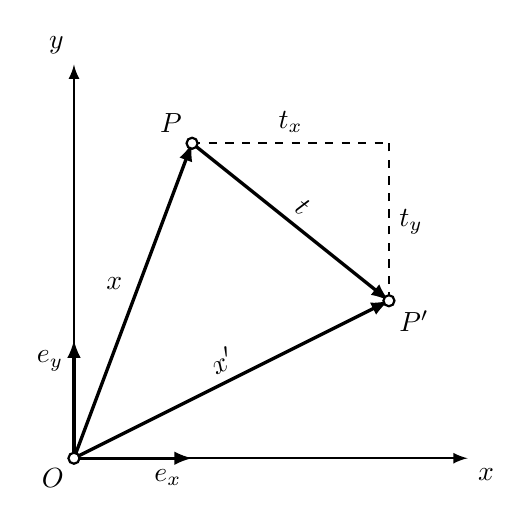
\begin{tikzpicture}
    %\sansmath
    %----------------------------------------------------------------------------------------%
    % Koordinaten
    %----------------------------------------------------------------------------------------%
    \coordinate (O) at (0,0);
    \coordinate (P1) at (1.5,4);
    \coordinate (P2) at (4,2);
    %----------------------------------------------------------------------------------------%
    % Koordinatenachsen
    %----------------------------------------------------------------------------------------%
    \begin{scope}[thick,->,>=latex]
    \draw (O) -- +(5,0) node[anchor=north west] {$x$};
    \draw (O) -- +(0,5) node[anchor=south east] {$y$};
    \end{scope}
    %----------------------------------------------------------------------------------------%
    % Einheitsvektoren
    %----------------------------------------------------------------------------------------%
    \begin{scope}[very thick,->,>=latex,scale = 1.5]
    \draw (O) -- +(1,0) node[anchor=north east] {$\boldsymbol{e_{x}}$};
    \draw (O) -- +(0,1) node[anchor=north east] {$\boldsymbol{e_{y}}$};
    \end{scope}
    %----------------------------------------------------------------------------------------%
    % Vektoren
    %----------------------------------------------------------------------------------------%
    \begin{scope}[very thick,->,>=latex]
    \draw (O) -- (P1) node [midway, anchor = south east] {$\boldsymbol{x}$};
    \draw (O) -- (P2) node [midway, sloped, above] {$\boldsymbol{x}^\prime$};
    \draw (P1) -- (P2) node [midway, sloped, above] {$\boldsymbol{t}$};
    \end{scope}
    %----------------------------------------------------------------------------------------%
    % Komponenten
    %----------------------------------------------------------------------------------------%
    \begin{scope}[thick, dashed]
    \draw (P1) -- (P2|-P1) node [midway, anchor = south] {$t_{x}$};
    \draw (P2) -- (P1-|P2) node [midway, anchor = west] {$t_{y}$};
    \end{scope}
    %----------------------------------------------------------------------------------------%
    % Punkte
    %----------------------------------------------------------------------------------------%
    \begin{scope}[thick,draw=black,fill=white]
    \filldraw (O) circle (2pt) node[anchor=north east] {$O$};
    \filldraw (P1) circle (2pt) node[anchor=south east] {$P$};
    \filldraw (P2) circle (2pt) node[anchor=north west] {$P^\prime$};
    \end{scope}
\end{tikzpicture}